\level{1}{Casi d'uso}
L’analisi del \insglo{capitolato}, l’incontro con il proponente e la discussione tra gli \insrole{Analisti} hanno portato all'individuazione dei casi d'uso riportati di seguito. 
I casi d'uso sono suddivisi in tre categorie, in quanto il progetto prevede la creazione di tre sistemi differenti:
\begin{description}
	\item[\insglo{Norris}] sono i casi d'uso inerenti alle funzionalità offerte dal \insglo{framework};
	\item[Applicazione \insglo{Android}] sono i casi d'uso inerenti all'utilizzo dell'applicazione \insglo{Android};
	\item[\insglo{Dashboard}] sono i casi d'uso inerenti all'utilizzo della \insglo{dashboard}.
\end{description}
Ogni caso d'uso è identificato da un codice univoco. La descrizione del modo in cui un caso d'uso viene identificato è rintracciabile nel documento \insdoc{Norme di Progetto v6.00}.\\
Si noti che nell'analisi dei casi d'uso viene utilizzato il concetto di attore. Un attore è qualsiasi cosa esterna al sistema che interagisca con esso. In particolare, un attore può rappresentare sia un utente umano sia un sistema esterno. È necessario dunque rimarcare che la differenza tra un attore e un utente è che il primo rappresenta il ruolo di un'entità esterna che interagisce con il sistema, mentre il secondo rappresenta in realtà una particolare classe di attori, quelli umani.\\
In seguito a queste considerazioni, è evidente come si debba mettere in relazione gli utenti descritti in precedenza con gli attori che vengono individuati nei casi d'uso espressi in seguito. Quindi, lo studio di ogni singolo sistema inizia con l'esplicazione della relazione che intercorre tra gli utenti e gli attori.

\level{2}{Norris}
	\level{3}{Relazione tra utenti e attori}
	Mettiamo in relazione gli utenti utilizzatori di \insglo{Norris} con gli attori che sono stati utilizzati nei seguenti casi d'uso. Si ricordi, infatti, che gli utenti non sono altro che una particolare classe degli attori.
	\begin{figure}[H]
		\centering
		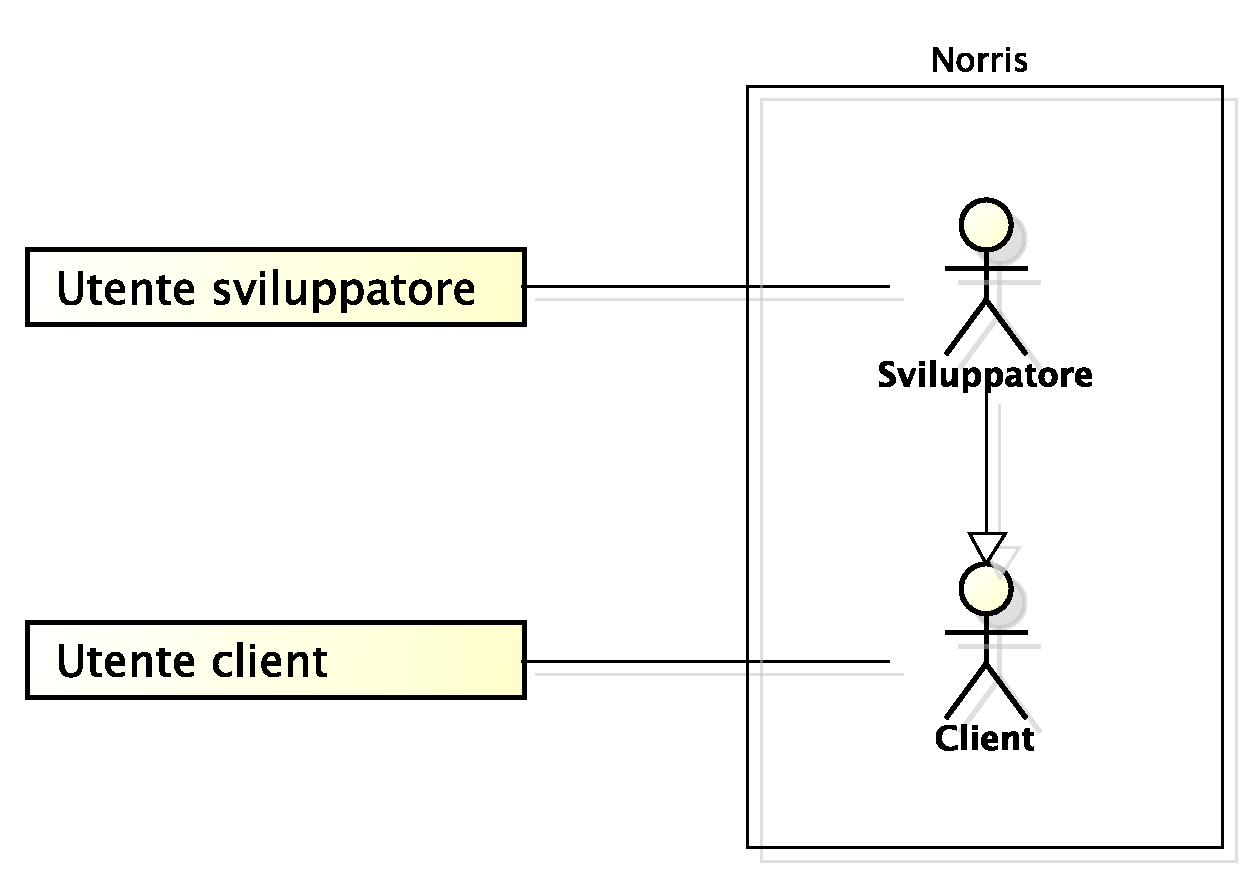
\includegraphics[scale=0.4]{Pics/UtentiAttoriNorris}
		\caption{Norris - Relazione tra utenti e attori}
	\end{figure}
	Si noti che gli attori individuati rappresentano anche sistemi ed entità non umane, nonostante il loro nome richiami quello degli utenti ad essi associati.
	\begin{itemize}
		\item L'attore che rappresenta il ruolo degli sviluppatori di istanze \insglo{Norris} è stato chiamato \emph{\insglo{Norris} developer}. Oltre a rappresentare l'utente ad esso associato, tale attore ingloba al suo interno tutte le applicazioni e i sistemi automatici in grado di modificare direttamente l'istanza di \insglo{Norris}.
		\item L'attore che rappresenta il ruolo degli sviluppatori di siti web è stato chiamato \emph{Web developer}. Oltre a rappresentare l'utente ad esso associato, tale attore ingloba al suo interno tutti i siti web che utilizzano grafici messi a disposizione da un \insglo{server} \insglo{Norris}.
		\item L'attore che rappresenta il ruolo degli sviluppatori di applicazioni lato \insglo{client} è stato chiamato \emph{App developer}. Oltre a rappresentare l'utente ad esso associato, tale attore ingloba al suo interno tutte le applicazioni e i sistemi automatici che utilizzano grafici messi a disposizione da un \insglo{server} \insglo{Norris}.
	\end{itemize}
	\input{UseCase/UCN.tex}

\level{2}{Applicazione Android}
	\level{3}{Relazione tra utenti e attori}
	Mettiamo in relazione gli utenti utilizzatori di dell'applicazione \insglo{Android} con gli attori che sono stati utilizzati nei seguenti casi d'uso. Si ricordi, infatti, che gli utenti non sono altro che una particolare classe degli attori.
	\begin{figure}[H]
		\centering
		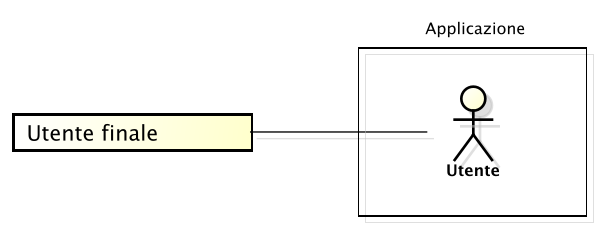
\includegraphics[scale=0.4]{Pics/UtentiAttoriApplicazione}
		\caption{Applicazione - Relazione tra utenti e attori}
	\end{figure}
	L'unico attore individuato (\emph{Utente}) coincide in questo caso con l'utente stesso dell'applicazione. È infatti previsto che sia solo l'utente umano a interagire con l'applicazione \insglo{Android}.
	\input{UseCase/UCA.tex}

\level{2}{Dashboard}
	\level{3}{Relazione tra utenti e attori}
	Mettiamo in relazione gli utenti utilizzatori della \insglo{Dashboard} con gli attori che sono stati utilizzati nei seguenti casi d'uso. Si ricordi, infatti, che gli utenti non sono altro che una particolare classe degli attori.
	\begin{figure}[H]
		\centering
		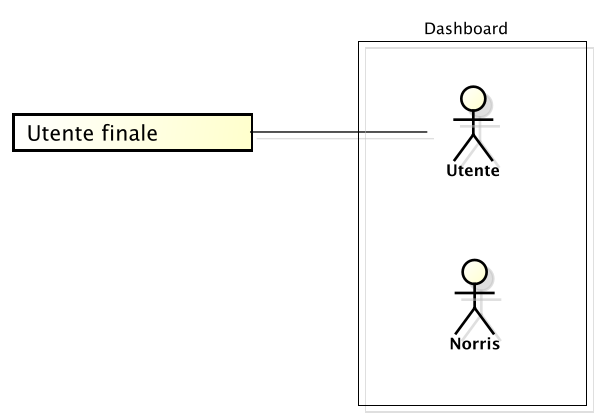
\includegraphics[scale=0.4]{Pics/UtentiAttoriDashboard}
		\caption{Dashboard - Relazione tra utenti e attori}
	\end{figure}
	Nel caso d'uso della \insglo{Dashboard}, l'attore principale (\emph{Utente}) coincide con l'utente stesso che fa uso della pagina. Infatti, è previsto che solo attori umani interagiscano con essa. L'attore secondario, invece, non è in relazione con alcun utente in quanto esso rappresenta un'istanza di \insglo{Norris} (che, ovviamente, non è un'entità umana).
	\input{UseCase/UCD.tex}
